\documentclass{beamer}
\usepackage{physics}
\usepackage{amsmath}
\usepackage{tikz}
\usepackage{mathdots}
\usepackage{yhmath}
\usepackage{cancel}
\usepackage{color}
\usepackage{siunitx}
\usepackage{array}
\usepackage{multirow}
\usepackage{amssymb}
\usepackage{textcomp, gensymb}
\usepackage{tabularx}
\usepackage{extarrows}
\usepackage{booktabs}
\usetikzlibrary{fadings}
\usetikzlibrary{patterns}
\usetikzlibrary{shadows.blur}
\usetikzlibrary{shapes}
\usepackage{listings}
\usepackage{hyperref}

\newcommand{\pair}[1]{\langle #1 \rangle}
\DeclareMathOperator{\ee}{e}
\DeclareMathOperator{\ii}{i}

%Information to be included in the title page:
\title{Numerical bootstrap}
\author{Jinyuan Wu}
\institute{Department of Physics, Fudan University}

\usetheme{Madrid}

\newcommand{\concept}[1]{\textbf{#1}}

\begin{document}

\frame{\titlepage}

\begin{frame}
\frametitle{Numerical methods for strongly correlated systems}

\textbf{Strongly correlated systems}

\begin{itemize}
    \item Fermi liquid: interaction correction of Fermi gas
    \item Strongly correlated systems: something non-perturbative happens
\end{itemize}

\textbf{Numerical approaches}

\begin{itemize}
    \item DQMC: discrete path integral and discrete Hubbard-Stratonovich transformation
    \item DMRG (MERA, PEPS): tensor network wave function ansatz
    \item Diagrammatic Monte-Carlo: stochastic summation of Feynman diagrams
    \item DMFT: self-energy correction + impurity model
\end{itemize}

\textbf{What's in common:} All with unobservable objects, be it the path integral or wave function or Feynman diagram or \dots 
%$\Rightarrow$ no hint about what goes wrong when they fail

\end{frame}

\begin{frame}
\frametitle{Introduction}

\textbf{What's bootstrap}

\begin{itemize}
    \item A model = expectations of all operators
    \begin{itemize}
        \item Hamiltonian/Lagrangian $\Leftrightarrow$ ``probability distribution''
        \item independent $\expval{O}$'s $\Leftrightarrow$ parameters in the model (``\concept{data}'')
    \end{itemize}
    
    \item Probability distribution $\Rightarrow$ Equality constraint on $\{\expval{O}\}$ without carrying out substantial calculation
    \begin{itemize}
        \item Trivial example: Wick theorem
        \item Conformal symmetry 
    \end{itemize}
    \item Inequality constraint $\Rightarrow$ allowed range of $\expval{O}$'s
    \begin{itemize}
        \item Positivity of $\expval{O^\dagger O}$
        \item Relaxed equational constraints
    \end{itemize}
    \item Obtaining estimation of physical quantities without the wave function/path integral (``out of nothing''): 
    hence the name \emph{bootstrap}
\end{itemize}

\vspace{1em}

\end{frame}

\begin{frame}
\frametitle{Example: conformal bootstrap}

\begin{itemize}
    \item The most famous example: \concept{conformal bootstrap}
    \item Constraints: (spinless) two-point function 
    \begin{equation}
        \expval*{\mathcal{O}(x) \mathcal{O}(y)} = \frac{1}{\abs*{x - y}^{2 \Delta_\mathcal{O}}},
    \end{equation}
    three-point function 
    \begin{equation}
        \begin{aligned}
            &\quad \langle\mathcal{A}(x) \mathcal{B}(y) \mathcal{C}(z)\rangle \\
            &= \frac{f_{\mathcal{A B C}}}{|x-y|^{\Delta_{\mathcal{A}}+\Delta_{\mathcal{B}}-\Delta_{\mathcal{C}}}|y-z|^{\Delta_{\mathcal{B}}+\Delta_{\mathcal{C}}-\Delta_{\mathcal{A}}}|z-x|^{\Delta_{\mathcal{C}}+\Delta_{\mathcal{A}}-\Delta_{\mathcal{B}}}}
        \end{aligned}
    \end{equation}
    Higher order correlation functions: OPEs. 
    \item Independent parameters: $\{\Delta_{\mathcal{O}}, l_{\mathcal{O}}, f_{\mathcal{A} \mathcal{B} \mathcal{C}}\}$
    \item Self-consistent conditions: determining the range of parameters
\end{itemize}

\end{frame}

\begin{frame}
\frametitle{Bootstrap for generic systems}

\textbf{How to perform bootstrap for a generic system?}    

\begin{itemize}
    \item The data: Correlation functions cannot be reduced to countably infinite parameters: 
    no $\{\Delta_{\mathcal{O}}, l_{\mathcal{O}}, f_{\mathcal{A} \mathcal{B} \mathcal{C}}\}$.
    
    \textbf{Solution} Store the normal-ordered $\{\expval{O_i}\}$ set (a basis of the operator space) with a cutoff. This is the data.
    Using equational constraints to reduce the size of data.

    Example:
    \begin{equation}
        \expval*{p x^3} = \expval*{x^3 p} - 3 \ii \expval*{x^2}.
    \end{equation}
    Data used: $\{ \expval*{x^3 p}, \expval*{x^2} \} \in \{\expval*{x^m p^n}\}$
\end{itemize}

\end{frame}

\begin{frame}
\frametitle{Bootstrap for generic systems}

\textbf{How to perform bootstrap for a generic system?}  

\begin{itemize}
    \item The equality constraints

    \textbf{Solution} $\rho = \ee^{- \beta H} / Z$, $\comm{\rho}{H} = 0$, then for all operators $O$
    \[
        \expval*{O H} = \trace (\rho(H) O H) = \trace(H \rho(H) O) = \trace(\rho(H) H O)  = \expval*{H {O}},
    \]
    \begin{equation}
        \expval*{\comm{O}{H}} = 0
    \end{equation}
    Similarly, suppose $C$ is a symmetry of the system, we have 
    \begin{equation}
        \expval*{\comm{O}{C}} = 0.
    \end{equation}
    There are linear constraints w.r.t the operator basis $\{O_i\}$.

    For energy eigenstates (i.e with definite but unknown $E$), we have 
    \begin{equation}
        \expval{O H} = E \expval{O}, \quad E = \expval{H}.
    \end{equation}
    This is a nonlinear constraint.
\end{itemize}

\end{frame}

\begin{frame}
\frametitle{Bootstrap for generic systems}

\textbf{Example of equality constraint} Suppose $H = x^2 + p^2 + x^4$, then 
\[
    \expval*{\comm{H}{xp}} = 0
\]    
gives linear constraint
\begin{equation}
    \expval*{p^2} - \expval*{x^2} - 2 \expval*{x^4} = 0,
\end{equation}
and 
\[
    \expval*{xp \cdot H} = E \expval*{xp}
\]
gives nonlinear constraint
\begin{equation}
    \begin{aligned}
        \expval*{xp^3} + \expval*{x^3 p} - 2 \ii \expval*{x^2} + \expval*{x^5 p} - 4 \ii \expval*{x^4} \\
        - \expval*{xp} \expval*{x^2} - \expval*{xp} \expval*{p^2} - \expval*{xp} \expval*{x^4} = 0.
    \end{aligned}
\end{equation}

\end{frame}

\begin{frame}
\frametitle{Bootstrap for generic systems}

\begin{itemize}
    \item The equality constraints together with the positivity constraint $\expval*{O^\dagger O} \geq 0$
    for every $O$ defines a feasible domain.
    \item This is an \concept{semidefinite programming (SDP)} problem: 
    \begin{equation}
        M_{ij} = \expval*{O_i^\dagger O_j} = \sum_k c^k_{ij} \expval*{O_k}, \quad M \geq 0.
    \end{equation} 
\end{itemize} 

\begin{columns}
    
\begin{column}{0.5\textwidth}
    \begin{itemize}
        \item $\expval*{\comm{O}{C}} = 0$: \concept{linear SDP}, convex feasible domain, 
        $\min \expval*{H} \Leftrightarrow$ ground state information
        \item $\expval*{OH} = \expval*{H} \expval*{O}$: \concept{nonlinear SDP}, nonconvex feasible domain; 
        a connected component = an eigenstate (or a continuous spectrum)
    \end{itemize}
\end{column}

\begin{column}{0.5\textwidth}
    \begin{center}
        

\tikzset{every picture/.style={line width=0.75pt}} %set default line width to 0.75pt        

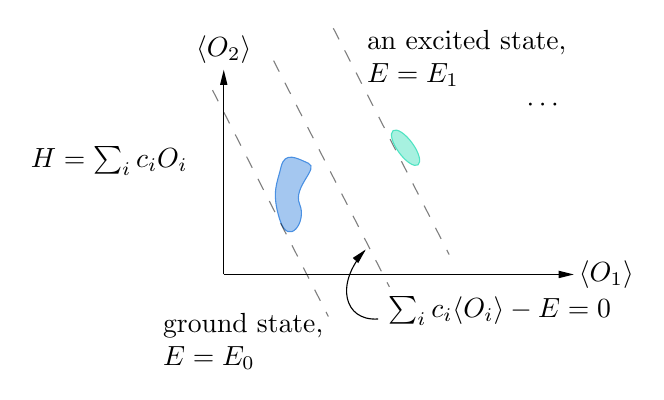
\begin{tikzpicture}[x=0.75pt,y=0.75pt,yscale=-0.6,xscale=0.6]
%uncomment if require: \path (0,353); %set diagram left start at 0, and has height of 353

%Straight Lines [id:da904255078328454] 
\draw    (177,246) -- (456,246) ;
\draw [shift={(458,246)}, rotate = 180] [fill={rgb, 255:red, 0; green, 0; blue, 0 }  ][line width=0.08]  [draw opacity=0] (12,-3) -- (0,0) -- (12,3) -- cycle    ;
%Straight Lines [id:da28860077544833507] 
\draw    (177,246) -- (177,83.73) ;
\draw [shift={(177,81.73)}, rotate = 90] [fill={rgb, 255:red, 0; green, 0; blue, 0 }  ][line width=0.08]  [draw opacity=0] (12,-3) -- (0,0) -- (12,3) -- cycle    ;
%Shape: Polygon Curved [id:ds05129166801576668] 
\draw  [color={rgb, 255:red, 74; green, 144; blue, 226 }  ,draw opacity=1 ][fill={rgb, 255:red, 74; green, 144; blue, 226 }  ,fill opacity=0.5 ] (223,159.73) .. controls (226,146.73) and (236,152.73) .. (245,156.73) .. controls (254,160.73) and (232,175.73) .. (238,189.73) .. controls (244,203.73) and (229,224.27) .. (222,202) .. controls (215,179.73) and (220,172.73) .. (223,159.73) -- cycle ;
%Straight Lines [id:da6483527344854445] 
\draw [color={rgb, 255:red, 0; green, 0; blue, 0 }  ,draw opacity=0.5 ] [dash pattern={on 4.5pt off 4.5pt}]  (168,98) -- (261,279.73) ;
%Straight Lines [id:da0036541181567224523] 
\draw [color={rgb, 255:red, 0; green, 0; blue, 0 }  ,draw opacity=0.5 ] [dash pattern={on 4.5pt off 4.5pt}]  (217,74.27) -- (310,256) ;
%Straight Lines [id:da34767057063343554] 
\draw [color={rgb, 255:red, 0; green, 0; blue, 0 }  ,draw opacity=0.5 ] [dash pattern={on 4.5pt off 4.5pt}]  (265,48.27) -- (358,230) ;
%Shape: Ellipse [id:dp302165402812995] 
\draw  [color={rgb, 255:red, 80; green, 227; blue, 194 }  ,draw opacity=1 ][fill={rgb, 255:red, 80; green, 227; blue, 194 }  ,fill opacity=0.5 ] (312.97,130.5) .. controls (310.07,132.62) and (312.21,140.48) .. (317.75,148.06) .. controls (323.29,155.64) and (330.13,160.08) .. (333.03,157.96) .. controls (335.93,155.84) and (333.79,147.98) .. (328.25,140.4) .. controls (322.71,132.81) and (315.87,128.38) .. (312.97,130.5) -- cycle ;
%Curve Lines [id:da7414078371933952] 
\draw    (301,281.73) .. controls (273.42,283.7) and (266.21,253.65) .. (289.9,227.21) ;
\draw [shift={(291,226)}, rotate = 133.09] [fill={rgb, 255:red, 0; green, 0; blue, 0 }  ][line width=0.08]  [draw opacity=0] (12,-3) -- (0,0) -- (12,3) -- cycle    ;

% Text Node
\draw (460,246) node [anchor=west] [inner sep=0.75pt]    {$\langle O_{1} \rangle $};
% Text Node
\draw (177,78.33) node [anchor=south] [inner sep=0.75pt]    {$\langle O_{2} \rangle $};
% Text Node
\draw (307,261.4) node [anchor=north west][inner sep=0.75pt]    {$\sum _{i} c_{i} \langle O_{i} \rangle -E=0$};
% Text Node
\draw (259,275) node [anchor=north east] [inner sep=0.75pt]   [align=left] {ground state,\\$\displaystyle E=E_{0}$};
% Text Node
\draw (290,97.27) node [anchor=south west] [inner sep=0.75pt]   [align=left] {an excited state,\\$\displaystyle E=E_{1}$};
% Text Node
\draw (418,103.4) node [anchor=north west][inner sep=0.75pt]    {$\cdots $};
% Text Node
\draw (20,141.4) node [anchor=north west][inner sep=0.75pt]    {$H=\sum _{i} c_{i} O_{i}$};


\end{tikzpicture}

    \end{center}    
\end{column}

\end{columns}

\end{frame}

\begin{frame}
\frametitle{Bootstrap for generic systems}

\textbf{Some technical aspects of the problem}

\begin{columns}
    \begin{column}{0.6\textwidth}
        \begin{itemize}
            \item \concept{Linear SDP} 
            \begin{itemize}
                \item $\expval*{\comm{H}{O}} = 0$, thermal states allowed
                \item Convex optimization\footnote[frame]{See \href{https://en.wikipedia.org/wiki/Semidefinite_programming}{Wikipedia}}, Linear objective $\Rightarrow$ minimum at the edge
                \item Mature solvers like SCS or CSDP\footnote[frame]{\href{https://github.com/cvxgrp/scs}{https://github.com/cvxgrp/scs}, \href{https://github.com/coin-or/Csdp}{https://github.com/coin-or/Csdp}}
            \end{itemize}
            \item \concept{Nonlinear SDP} 
            \begin{itemize}
                \item $\expval*{{H}{O}} = E \expval*{O}$, there are optimization variables in $E$, eigenstates only
                \item No solver mature enough\footnote[frame]{See the discussion before Sec.~1.1 in \href{https://arxiv.org/abs/2108.04830}{arXiv 2108.04830}. Also, no nonlinear solver supporting SDP is listed in \href{https://jump.dev/JuMP.jl/stable/installation/}{the solver list of JuMP.jl}.}
            \end{itemize}
        \end{itemize} 
    \end{column}
    \begin{column}{0.4\textwidth}
        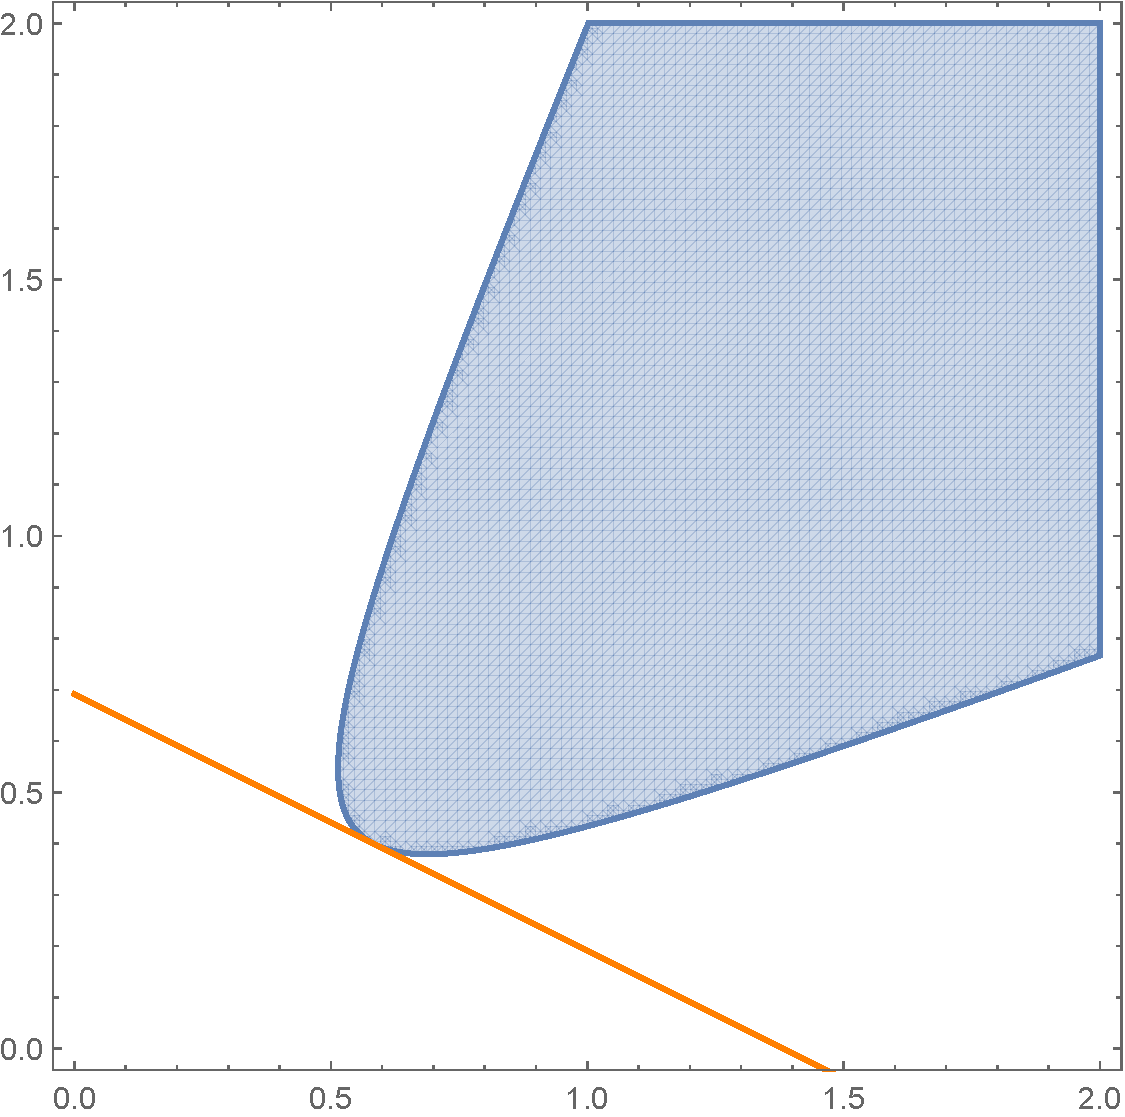
\includegraphics[width=\textwidth]{jump-toy-2-benchmark-feasible-domain-and-result.pdf}
    \end{column}
\end{columns}

\end{frame}

\begin{frame}
\frametitle{Bootstrap for generic systems}

\textbf{The procedure of numerical bootstrap}   

Input data:
\begin{itemize}
    \item $N$ basis operators $\{O_i\}$, normal ordered with a length cutoff
    \item Commutation rules, normal ordering rules, etc. so that $O_i O_j$ can be expanded in terms of $\{O_i\}$
    \item Data of equality constraints: Hamiltonian, symmetry, etc.
\end{itemize}

Building the optimization problem:
\begin{enumerate}
    \item Declare $N$ variables $\{X_i\}$, $X_i = \expval*{O_i}$ after optimization
    \item Impose equality constraints on $\{X_i\}$ according to e.g. $\expval*{\comm{H}{O}} = 0$ 
    \item Imposing semidefinite constraint on $M_{ij} = \expval*{O_i^\dagger O_j}$ (expanded into linear combination of $\{X_i\}$)
\end{enumerate}

\end{frame}

\begin{frame}
\frametitle{Bootstrap for generic systems}

\textbf{Why we need numerical bootstrap}

\begin{itemize}
    \item Because it doesn't fail with strong non-perturbative effects.\footnote{\href{https://arxiv.org/abs/2108.11416}{arXiv 2108.11416}}
    \item Because if done correctly, it gives the \emph{lower} bound of ground state energy
    \begin{itemize}
        \item Density matrix = linear functional $\mathcal{F}$ from operators to numbers
        \item Predicted $E_0$ = $\min_{\mathcal{F} \text{constrained}} \mathcal{F}[H]$
        \item Real ground state also constrained $\Rightarrow$ real $E_0 \geq $ predicted $E_0$
        \item Upper and lower bounds for all physical quantities:
        \begin{equation}
            \min_{E_\text{lb} \leq \expval*{H}_\rho \leq E_\text{ub}} \expval{O}_\rho \leq \expval*{O}_{\rho_0} \leq \max_{E_\text{lb} \leq \expval*{H}_\rho \leq E_\text{ub}} \expval{O}_\rho
        \end{equation}
    \end{itemize}
\end{itemize}    

\end{frame}

\begin{frame}
\frametitle{Examples}

\textbf{Anharmonic oscillator and Hubbard model}

\begin{itemize}
    \item Main topics of my thesis
\end{itemize}

\textbf{Double-well potential}\footnote{See \href{https://arxiv.org/abs/2108.11416}{arXiv 2108.11416}}

\begin{itemize}
    \item Non-perturbative: instanton effect
    \item Solved in a similar way of the anharmonic oscillator
    \item Dilute instanton approximation works with two wells well separated
\end{itemize}

\textbf{Matrix model}\footnote{See \href{https://arxiv.org/pdf/2108.04830.pdf}{arXiv 2108.04830} and \href{https://arxiv.org/abs/2004.10212}{arXiv 2004.10212}}

\begin{itemize}
    \item Hard to solve otherwise
    %\item A specific case associated with $M$-theory\footnote{\href{https://arxiv.org/abs/hep-th/9610043}{arXiv hep-th 9610043}}
    \item (Inherent) nonlinear constraints
    \begin{itemize}
        \item Relaxed bootstrap in Sec.~4 in \href{https://arxiv.org/pdf/2108.04830.pdf}{arXiv 2108.04830}
        \item trust-region sequential SDP in \href{https://github.com/hanxzh94/matrix-bootstrap}{Xizhi Han's code}
    \end{itemize}
\end{itemize}

\end{frame}

\begin{frame}
\frametitle{Example: $x^4$ anharmonic oscillator}

The anharmonic oscillator\footnote{The example is provided in \href{https://arxiv.org/abs/2004.10212}{arXiv 2004.10212}}: famous failure of perturbation theory\footnote{Carl M. Bender and Tai Tsun Wu, Anharmonic Oscillator. Phys. Rev. 184, 1231.}
\begin{equation}
    H = x^2 + p^2 + g x^4.
\end{equation}

\begin{itemize}
    \item Equality constraints from symmetry: $x \to -x$ $\Rightarrow$ $\expval*{x^n} = 0$ with odd $n$
    \item Equality constraints from Hamiltonian:
    \begin{itemize}
        \item $\mathcal{O}=x^{s}$ and $\mathcal{O}=x^{t} p$ in $\langle[H, \mathcal{O}]\rangle=0$ 
        \item $\mathcal{O}=x^{t-1}$ in $\langle\mathcal{O} H\rangle=E\langle\mathcal{O}\rangle$
    \end{itemize}
    \item So finally we have
        \begin{equation}
            \begin{aligned}
                &E=2\left\langle x^{2}\right\rangle+3 g\left\langle x^{4}\right\rangle, \\
                &4 t E\left\langle x^{t-1}\right\rangle +t(t-1)(t-2)\left\langle x^{t-3}\right\rangle -4(t+1)\left\langle x^{t+1}\right\rangle \\
                &\quad -4 g(t+2)\left\langle x^{t+3}\right\rangle=0 
            \end{aligned}
        \end{equation}
    \item Only independent variables: $\{\expval*{x^2}, E\}$, so nonlinear SDP is possible
    \item SDP constraint: $M_{ij} = \expval*{x^{i+j}}, M \geq 0, 0 \leq i, j \leq K$
\end{itemize}

\end{frame}

\begin{frame}[fragile]
\frametitle{Example: $x^4$ anharmonic oscillator}

\begin{itemize}
    \item Reproduce Fig.~1 in \href{https://arxiv.org/abs/2004.10212}{arXiv 2004.10212} by brutal force searching
    \item Numerical bootstrap can be quite precise! (high resolution Mathematica plotting required to find the allowed region)
\end{itemize}

\begin{columns}
    
    \begin{column}{0.5\textwidth}
        \lstset{language=Mathematica, basicstyle=\tiny, xleftmargin=-40pt}
        % Code from oscillator-simple-prototype\2022-1-20.nb
        \begin{lstlisting}
            expectedX[0] := 1;
            expectedX[2] := x2;
            expectedX[4] := 1/(3 g) (E0 - 2 x2);
            expectedX[u_?EvenQ] := 
            1 / (4 g ((-3 + u) + 2)) * 
            (4 (-3 + u) E0 expectedX[(-3 + u) - 1] 
            + (-3 + u) ((-3 + u) - 1) ((-3 + u) - 2) 
                expectedX[(-3 + u) - 3] 
            - 4 ((-3 + u) + 1) expectedX[(-3 + u) + 1]);

            matPositive[K_] := 
            Table[expectedX[i+j], {i, 0, K}, {j, 0, K}];

            RegionPlot[
            AllTrue[Eigenvalues[matPositive[9] /. g -> 1], 
                # >= 0 &], 
            {E0, 1.35, 1.44}, {x2, 0.294, 0.311}, 
            PlotPoints -> 100]
        \end{lstlisting}
    \end{column}

    \begin{column}{0.5\textwidth}
        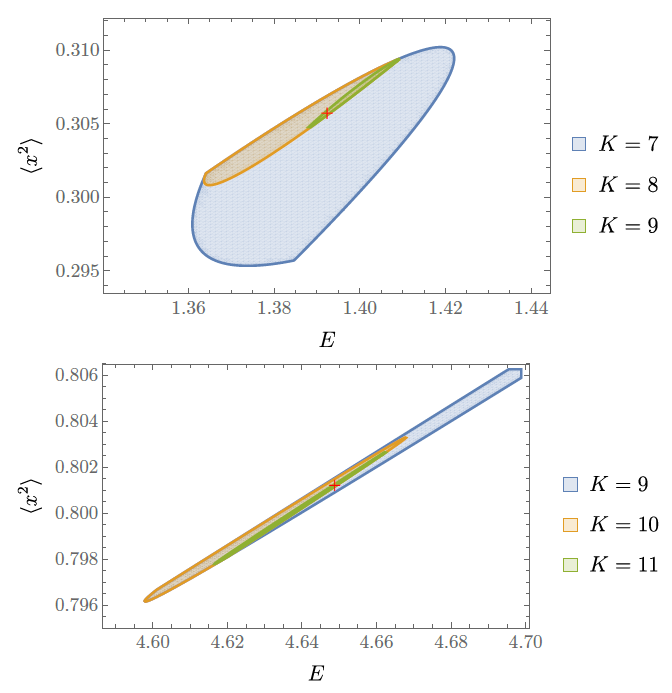
\includegraphics[width=\textwidth]{oscillator-bootstrap-feasible-domains.PNG}
    \end{column}
\end{columns} 

\end{frame}

\begin{frame}
\frametitle{Example: $x^4$ anharmonic oscillator}

\textbf{Benchmark}

\begin{itemize}
    % program: oscillator-simple-prototype\stationary-schrodinger.jl
    \item Solving the Schr\"{o}dinger equation with finite difference method with $\Delta x = 0.05$: $E_0 = 1.3919$
    % program: oscillator-simple-prototype\2022-1-20.nb
    \item Numerical bootstrap with $K=11$: $E_0 = 1.3922$
\end{itemize}  

\end{frame}

\begin{frame}
\frametitle{Example: $x^4$ anharmonic oscillator}

\textbf{Linear SDP}

\begin{itemize}
    \item Solver: JuMP and COSMO\footnote{\href{https://jump.dev/JuMP.jl/stable/}{https://jump.dev/JuMP.jl/stable/}, \href{https://oxfordcontrol.github.io/COSMO.jl/stable/}{https://oxfordcontrol.github.io/COSMO.jl/stable/}}
    \item Operator algebra: McCoy formula
    \begin{equation}
        {\left[{ {x}}^{n},{ {p}}^{m}\right]=\sum _{k=1}^{\min \left(m,n\right)}{{\frac {-\left(-i\hbar \right)^{k}n!m!}{k!\left(n-k\right)!\left(m-k\right)!}}{ {x}}^{n-k}{ {p}}^{m-k}}}.
    \end{equation}
    \item Operator basis and cutoff: $\{x^m p^n\}$, where $0 \leq m, n \leq 2L$ 
    \item Hence for $O_i = x^m p^n$ in $M_{ij} = \expval*{O_i^\dagger O_j}$, $0 \leq m, n \leq L$
    \item COSMO only support real variables $\Rightarrow$ Declare two JuMP variables for $\Re O$ and $\Im O$ (odd $m + n$ $\Rightarrow$ zero expectation, odd $n$ $\Rightarrow$ imaginary, even $n$ $\Rightarrow$ real),
    \begin{equation}
        M_{ij} \to \Re(M_{ij}) \pmqty{1 & 0 \\ 0 & 1} + \Im(M_{ij}) \pmqty{0 & -1 \\ 1 & 0}.
    \end{equation}
\end{itemize}

\end{frame}

\begin{frame}
\frametitle{Example: $x^4$ anharmonic oscillator}

\textbf{Result of linear SDP}

\begin{itemize}
    \item Successful when $L$ is small
    \item But when $L$ is 4\dots Severe convergent problem!
    \item Both stationary Schr\"{o}dinger equation and nonlinear SDP estimate $E \approx 1.392, \expval*{x^2} \approx 0.306$. Not sure whether 
    $L=4$ converges.
    \item $L=5$ takes 80000000 iterations and still doesn't converge.
    \item Only COSMO works for $L=4$; SCS and CSDP report infeasibility
    \item False convergence when \texttt{eps\_rel} is not small enough (\num{1e-5} not enough; \num{1e-10} works for $L=4$)
\end{itemize}

\begin{center}
    \begin{tabular}{cccc}
        \toprule
          $L$ & $E$ & $\expval*{x^2}$ & time consumption \\
        \midrule
          2 & 1.381  & 0.313 & 0.752s, 958 iterations  \\
          3 & 1.387  & 0.305 & 2.501s, 1194 iterations \\
          4 & 1.394  & 0.306 & 172375s, 79461867 iterations  \\
        \bottomrule
    \end{tabular}
\end{center}

\end{frame}

\begin{frame}
\frametitle{Example: $x^4$ anharmonic oscillator}

\textbf{Possible reasons of the convergence problem}

\begin{itemize}
    \item Too much time is spent on tightening the constraints. Hints:
    \begin{itemize}
        \item In the solver log of the $L=4, 5$ cases, first energy goes down and residue goes up, then residue goes down and energy goes up, \dots
        \item False convergence
        \item Solution: eliminate some variables in the optimization problem
    \end{itemize}
    \item Float precision not enough, introducing fluctuation. Hints:
    \begin{itemize}
        \item This is the case in conformal bootstrap.
        \item Diagnosis: using less precise floats for $L= 2, 3$ and checking if the problem recurs.
        \item Solution: same as conformal bootstrap
    \end{itemize}
    \item The scheme
    \begin{equation}
        M_{ij} \to \Re(M_{ij}) \pmqty{1 & 0 \\ 0 & 1} + \Im(M_{ij}) \pmqty{0 & -1 \\ 1 & 0}
    \end{equation}
    is bad. Hints:
    \begin{itemize}
        \item No convergence problem in Hubbard model. (strange but true \dots)
        \item Solution: rephrasing the anharmonic oscillator in terms of the creation and annihilation operators
    \end{itemize}
\end{itemize}

\end{frame}

\begin{frame}
\frametitle{Example: Hubbard model}

\concept{Hubbard model}\footnote{\href{https://arxiv.org/abs/2006.06002}{arXiv 2006.06002}}
\begin{equation}
    H = - t \sum_{\pair{\vb*{i}, \vb*{j}}, \sigma} c^\dagger_{\vb*{i} \sigma} c_{\vb*{j} \sigma} + U \sum_{\vb*{i}} n_{\vb*{i} \uparrow} n_{\vb*{j} \downarrow}
\end{equation}
is probably the most important strongly correlated electronic model.

\begin{itemize}
    \item Half filling: small $U$ $\Rightarrow$ Fermi liquid, large $U$ $\Rightarrow$ Heisenberg model (Mott transition, spin-charge separation)
    \item Doping: t-J model, superconductivity
    \item Problems of various numerical approaches:
    \begin{itemize}
        \item DQMC: sign problem when doped away from half-filling, can be tackled in some case\footnote{\href{https://arxiv.org/abs/2204.08777}{arXiv 2204.08777}} but no generic solution\footnote{\href{https://arxiv.org/abs/cond-mat/0408370}{arXiv cond-mat 0408370}} 
        \item DMRG: works well in 1D but slow in 2D 
        %\item Finite size effect
    \end{itemize}
\end{itemize}

\end{frame}

\begin{frame}
\frametitle{Example: Hubbard model}

\textbf{Linear SDP}

\begin{itemize}
    \item Solver: JuMP and COSMO
    \item Operator algebra: QuantumAlgebra.jl\footnote{\href{https://github.com/jfeist/QuantumAlgebra.jl}{https://github.com/jfeist/QuantumAlgebra.jl}}
    \item Operator basis and cutoff: normal ordered $\{c^\dagger_{\vb*{i}_{1} \sigma_1} c^\dagger_{\vb*{i}_2 \sigma_2} \cdots c_{\vb*{i}_n \sigma_n}\}$, $n + \sum_{k=1}^n \| \vb*{i}_k \|_1 \leq K$
    \item One JuMP variable for one operator $\Leftarrow$ the whole model is real
    \item Expectations of operators that do not keep particle number (e.g. $c^\dagger_{1 \uparrow} c^\dagger_{2\uparrow} c^\dagger_{3\uparrow} c_{1 \uparrow}$) and total spin (e.g. $c^\dagger_{1 \uparrow} c_{1 \downarrow}$) are zero
    \item Translational and inversion symmetry: $\expval*{c_{1 \uparrow}^\dagger c_{1 \uparrow}} = \expval*{c_{2 \uparrow}^\dagger c_{2 \uparrow}}$
    \item Electron filling: need to be explicitly imposed
    \begin{itemize}
        \item half filling $\Rightarrow$ $\expval*{n_1} = \expval*{n}_2 = \cdots = 1$
        \item doping $\Rightarrow$ $\expval*{n_1} = \expval*{n}_2 = \cdots = 0.75$, etc.
        \item \emph{Not} done by chemical potential (which is the case in DQMC but not in DMRG)
    \end{itemize}
\end{itemize}

\end{frame}

\begin{frame}
    \frametitle{Example: Hubbard model}

    \textbf{DMRG benchmark}

    \begin{itemize}
        \item Using ITensor's fixed quantum number DMRG to find reference values
        \item The DMRG solution is in the feasible domain (so the implementation is correct)
    \end{itemize}
\end{frame}

\begin{frame}
\frametitle{Example: Hubbard model}

\textbf{1D square lattice}

\begin{center}
    \begin{tabular}{cccccc}
        \toprule
        \multicolumn{2}{c}{$n_i=1$}                                 & $U=4$   & $U=6$   & $U=8$   & $U=10$  \\
        \midrule
        \multirow{2}{*}{$K=10$} & $E$                               & -0.6202 & -0.4580 & -0.3574 & -0.2913  \\
                                & $n_{i \uparrow} n_{i \downarrow}$ &  0.1071 &  0.0639 &  0.0406 &  0.0275 \\
        \midrule
        \multirow{2}{*}{$K=12$} & $E$                               & -0.6049 & -0.4466 & -0.3486 & -0.2842  \\
                                & $n_{i \uparrow} n_{i \downarrow}$ &  0.1027 &  0.0618 &  0.0394 &  0.0267  \\
        \midrule
        \multirow{2}{*}{Exact}  & $E$                               & -0.5737 & -0.4201 & -0.3275 & -0.2672  \\
                                & $n_{i \uparrow} n_{i \downarrow}$ &  0.1002 &  0.0582 &  0.0366 &  0.0248  \\
        \bottomrule
    \end{tabular}
\end{center}

\begin{itemize}
    \item Approximately correct, but not as good as Xizhi Han's results
    \item Converges rather quickly: 20 minutes for $K=12$, \num{7e5} variables
    \item Larger $U$ $\Rightarrow$ smaller absolute error, larger relative error 
\end{itemize}

\end{frame}

\begin{frame}
\frametitle{Example: Hubbard model}

\textbf{1D square lattice}

\begin{itemize}
    \item Accuracy with various $U$
    \begin{itemize}
        \item Expected: large $U$ $\Rightarrow$ localized electrons, so with our local operators large $U$ means higher accuracy
        \item Observed: Larger $U$ $\Rightarrow$ smaller absolute error, larger relative error 
        \item What's the correct way to evaluate the accuracy of numerical bootstrap?
    \end{itemize}
    \item Main performance bottleneck: \emph{before} optimization, the step turning QuantumAlgebra.jl operators
    into JuMP variables
\end{itemize}

\end{frame}

\begin{frame}
\frametitle{Example: Hubbard model}

\textbf{1D square lattice with doping}

\begin{center}
    \begin{tabular}{cccccc}
        \toprule
        \multicolumn{2}{c}{$n_i=0.5$}                                 & $U=4$   & $U=6$   & $U=8$   & $U=10$  \\
        \midrule
        \multirow{2}{*}{$K=12$} & $E$                               & -0.7830 & -0.7593 & -0.7444 & -0.7342  \\
                                & $n_{i \uparrow} n_{i \downarrow}$ &  0.0168 &  0.0102 &  0.0068 &  0.0048  \\
        \midrule
        \multirow{2}{*}{DMRG}  & $E$                               & -0.7534 & -0.7243 & -0.7059 & -0.6939  \\
                                & $n_{i \uparrow} n_{i \downarrow}$ &  0.0189 &  0.0114 &  0.0075 &  0.0052  \\
        \bottomrule
    \end{tabular}
\end{center}

\begin{itemize}
    \item Comparison of accuracy between half filling and hole doping 
    \begin{itemize}
        \item Errors larger than half filling
        \item Expected: hole doping $\Rightarrow$ iterant electrons, whose behavior can't be captured by local operators $\Rightarrow$ poorer accuracy \checkmark
    \end{itemize}
    \item $U$ increase $\Rightarrow$ relative and absolute errors increase?? 
\end{itemize}

\end{frame}

\begin{frame}
\frametitle{Example: Hubbard model}

\textbf{2D square lattice}    

\begin{center}
    \begin{tabular}{cccccc}
        \toprule
        \multicolumn{2}{c}{$n_i=1$}                                 & $U=2$   & $U=4$   & $U=6$   & $U=8$  \\
        \midrule
        \multirow{2}{*}{$K=8$}     & $E$                               & -1.3164 & -1.0491 & -0.8626 & -0.7276  \\
                                    & $n_{i \uparrow} n_{i \downarrow}$ &  0.1602 &  0.1105 &  0.0784 &  0.0576  \\
        \midrule
        \multirow{2}{*}{DMRG}  & $E$                               & -1.176(1) & -0.8605(5) & -0.6565(1) & -0.5241(1)  \\
                                    & $n_{i \uparrow} n_{i \downarrow}$ &  0.188(1) &  0.126(1) &  0.0809(3) &  0.0539(1)  \\
        \bottomrule
    \end{tabular}
\end{center}

\begin{itemize}
    \item Time consumption gets larger (no real large-scale results)
    \item Error analysis
    \begin{itemize}
        \item The absolute error of $E$ as $U$ shows an increasing tendency (the relative error goes all the way higher)
        \item The absolute error of the double occupation decreases, and the relative error shows a decreasing tendency
        \item Expected: larger $U$ $\Rightarrow$ smaller error 
        \item Possible reason: energy bound is not very tight 
    \end{itemize}
    
\end{itemize}

\end{frame}

\begin{frame}
\frametitle{Conclusion}

\begin{itemize}
    \item Verify the result of nonlinear SDP bootstrap for anharmonic oscillator
    \item Linear SDP for anharmonic oscillator and convergence problem
    \item Linear SDP for Hubbard model, 1D, 1D doped and 2D, and error analysis
\end{itemize}    

\end{frame}

\begin{frame}
\frametitle{Future prospects}

\begin{itemize}
    \item Symmetry breaking: so the ground state $\rho$ is not a function of $H$: 
    \begin{equation}
        \lim_{\beta \to \infty} \frac{1}{Z} \ee^{- \beta H} = \frac{1}{2} (\dyad{\uparrow} + \dyad{\downarrow}) \neq \underbrace{\dyad{\uparrow}}_{\text{true ground state}} 
    \end{equation}
    \item Bootstrapping spin models: Heisenberg model, lattice frustration, next neighbor interaction induced frustration, spin liquids, etc.
    \item Bootstrapping a \emph{class} of models (e.g. ``all possible QM models'')
    \begin{itemize}
        \item Extending what is done in conformal bootstrap (e.g. ``all possible CFTs made by $\sigma$ and $\epsilon$'') to all kind of models
    \end{itemize}
    \item Extracting thermal information from $\expval*{\comm{O}{H}} = 0$ bootstraps
    \begin{itemize}
        \item What's the entropy? 
        \item What's the temperature in terms of operator expectations?
    \end{itemize}
    \item What constraints are effective? (Important for scaling up and interpretation)
    \begin{itemize}
        \item Can wave function ansatz (e.g. DMRG) provide some hints?
        \item Constraints that are ``almost'' violated are the most important?
        \item \href{https://arxiv.org/abs/2205.12325}{arXiv 2205.12325}: bootstrap and perturbation theory
    \end{itemize}
\end{itemize}

\end{frame}

\end{document}